\documentclass[a4paper, twoside]{article}

\usepackage{multirow}
\usepackage{multicol}
%\usepackage[T1]{fontenc}
%\usepackage[latin9]{inputenc}
%\usepackage{babel}
%\usepackage{alltt}
%\usepackage{comment}
%\usepackage{multirow}
%\usepackage{graphicx}

% -----------------
% --- comments: ---
% -----------------

\newcommand{\notethis}[1]{
  \color{red}
  \vspace{0.3cm}
  \noindent\makebox[\linewidth]{\rule{\paperwidth}{0.4pt}}\\
  {\sc NOTE - } #1\\
  \noindent\makebox[\linewidth]{\rule{\paperwidth}{0.4pt}}\\
  \vspace{0.3cm}
  \color{black}
}

% ------------------
% --- listings: ---
% ------------------

\usepackage{url}
\usepackage{listings}
\usepackage{color}
\usepackage{amssymb}
\usepackage{framed}
\usepackage{graphicx} 
\usepackage{caption} 
\captionsetup{compatibility=false}
\usepackage{subcaption}
\usepackage{fancyvrb}
\usepackage{verbatimbox}
\usepackage{verbatim}
\usepackage{fancyvrb}
\usepackage{apalike}
\usepackage{SCITEPRESS}

\definecolor{light-gray}{gray}{0.95}

\lstdefinelanguage{K}{
  morekeywords={package,import,class,unique,extends,with,match,new,if,then,else,while,for,yield,val,var,this,case,type,implicit,private,protected,abstract,final, req, Int, String, Bool, fun, pre, post},
  otherkeywords={&,\{,\},_*},
  literate=
      {\#\#}{{$\oplus\;$}}2
      {|->}{{$\longmapsto\;$}}2
      {-->}{{$\Longrightarrow\;$}}2
      {->}{{$\rightarrow\;$}}2
      {~}{{$\sim\;$}}2
      {>>}{{$\gg$}}2
      {++}{{$++$}}2
      {|==}{{$\models$}}2
  ,
  sensitive=true, 
  morecomment=[l]{//}, 
  morecomment=[s]{/*}{*/},
  stringstyle=\ttfamily,
  numbers=left,   
  numberstyle=\footnotesize, 
}

\lstdefinelanguage{SMT}{
  morekeywords={define,declare,sort,const,fun,datatypes,assert,forall,exists,and,or,ite,select,Int,Real,Bool,Array},
  sensitive=true, 
  morecomment=[l]{;}, 
  stringstyle=\ttfamily,
%  numbers=none,   
%  numberstyle=\footnotesize, 
}

 
% --- Referring to code: ---

\newcommand{\name}[1]{{\em #1}}
%\newcommand{\code}[1]{\texttt{#1}}
\newcommand{\issue}[2]{{\bf ** #1: #2}}

\newcommand{\Klang}{{K}}
\newcommand{\tracecontract}{{TraceContract}}
\newcommand{\logfire}{{LogFire}}
\newcommand{\vdm}{VDM}
\newcommand{\vdmpp}{\vdm$^{++}$}
\newcommand{\asml}{Asml}
\newcommand{\raiselang}{Raise}
\newcommand{\rsl}{RSL}
\newcommand{\zlang}{Z}
\newcommand{\alloy}{Alloy}
\newcommand{\clear}{Clear}
\newcommand{\eiffel}{Eiffel}
\newcommand{\dafny}{Dafny}
\newcommand{\whythree}{Why3}
\newcommand{\whyml}{WhyML}
\newcommand{\eml}{EML}
\newcommand{\specsharp}{SpeC$^{\#}$}
\newcommand{\java}{Java}
\newcommand{\clang}{C}
\newcommand{\scala}{Scala}
\newcommand{\sml}{SML}
\newcommand{\ml}{ML}
\newcommand{\haskell}{Haskell}
\newcommand{\fortress}{Fortress}
\newcommand{\python}{Python}
\newcommand{\ocaml}{Ocaml}
\newcommand{\jml}{JML}
\newcommand{\uml}{UML}
\newcommand{\sysml}{SysML}
\newcommand{\ltl}{LTL}
\newcommand{\pvs}{PVS}
\newcommand{\isabelle}{Isabelle}
\newcommand{\coq}{Coq}
\newcommand{\boogie}{Boogie}
\newcommand{\zthree}{Z3}
\newcommand{\ems}{EMS}
\newcommand{\antlr}{ANTLR}
\newcommand{\slam}{SLAM}
\newcommand{\spin}{SPIN}
\newcommand{\promela}{Promela}{

\newcommand*{\scaleFactor}{0.75}

% \lstset{language=K,numbers=left,numberstyle=\scriptsize,numbersep=-21pt}
\lstset{language=K}


\begin{document}

\title{K: A Wide Spectrum Language for\\ Modeling, Programming, and Analysis\thanks{ 
%\title{Towards a Textual Language for SysML\thanks{ 
%\title{Towards a Textual Language for\\ Model Based Systems Engineering\thanks{ 
The research was carried out at the Jet Propulsion
Laboratory, California Institute of Technology, under a contract
with the National Aeronautics and Space
Administration. \copyright\ 2015 California Institute of
Technology. Government sponsorship acknowledged.}}

\author{\authorname{Klaus Havelund, Rahul Kumar, Chris Delp and
    Bradley Clement} \affiliation{ Jet Propulsion Laboratory,
    California Institute of Technology, California, USA }
  \email{\{klaus.havelund, rahul.kumar, Christopher.L.Delp,
    Bradley.J.Clement\}@jpl.nasa.gov} }


\begin{abstract}

The formal methods community has over the years proposed various 
formally founded specification languages based on predicate logic 
and set theory. At the same time the model-based engineering community 
has proposed less formally founded graphical formalisms such as UML and 
SysML. We report on an effort to formally ground SysML in a textual 
formal language, named K, supporting classes, multiple inheritance, predicate 
logic and set theory. K contains programming constructs, and can thus be 
considered as a  wide-spectrum modeling and programming language. We further 
explain the translation of a subset of this textual language to the input 
language of the SMT-LIB standard, and the application of Z3 for analysis 
of the generated SMT-LIB formulas. The entire effort is part of a larger 
effort to develop a general purpose SysML development framework for designing 
systems, currently supporting the design of NASA's planned 2022 mission to 
Jupiter's Moon Europa. 

\end{abstract}


\keywords{Modeling, programming, constraints, refinement,
  verification, SMT, analysis.}


\onecolumn \maketitle \normalsize \vfill

\section{Introduction}
\label{sec:introduction}

Modeling is the activity of formulating an abstract description of a
system to be implemented (or possibly already implemented). Modeling
includes such activities as requirements capture in the initial phases
and design of higher-level architectural decisions in later
stages. Modeling has been studied by various communities, of which at
least two can be identified: the model-based engineering community and
the formal methods community. The {\em model-based engineering}
community has suggested graphical modeling languages such as UML
\cite{uml} and SysML \cite{sysml}, a variant of UML.  Both have been
designed by the OMG (Object Management Group) technology standards
consortium. SysML is meant for systems development more broadly
considered, including physical systems as well as software systems, in
contrast to UML, which is mainly meant for software development. These
graphical formalisms have received a high degree of popularity in
industry due to their two dimensional format, also sometimes referred
to popularly as {\em boxology}: boxes and arrows. However, drawbacks
of these formalisms include lack of precise semantics, lack of
analysis capabilities, tedious GUI operations, requiring lots
of visual real estate even for simple models, as well as large volumes
of technologies. Learning UML and SysML is not just learning very
large languages, it is also learning a large set of additional tools
needed to work with models. We formulate the hypothesis that some of these
drawbacks in part are due to the lack of a simple textual language, at
a size comparable to a programming language, underlying the
graphical notations.

From an even earlier point in time, since the 1960s, the {\em
  formal methods} community, part of the computer science community,
and closely connected to the programming language community, has
proposed numerous formally founded specification languages. Several of
these are based on predicate logic and set theory. These languages
are, compared to UML and SysML, concise, small, well defined in the
form of semantics, and in recent time well supported with analysis
capabilities. The obvious observation is that it might be fruitful to
study the interaction between the two classes of formalisms. Consider
furthermore that programming languages are gaining in abstraction,
such as for example combining object-oriented and functional
programming. An example is Scala, which has many commonalities with very early formal
specification languages, such as for example VDM \cite{vdm78}, and
specifically its object-oriented variant VDM$^{++}$
\cite{vdmplusplus05}.  The study should therefore include the
interaction between the graphical formalisms, the formal methods
modeling languages, and programming languages.

We report on an effort to formally ground SysML in a textual
formal specification language, named K (Kernel language), designed
specifically for this purpose.  
Our initial focus is on specifying and analyzing class diagrams
with constraints. K supports object-oriented concepts
such as classes, multiple inheritance, and object instances. The
contents of classes can be typed values, including functions, and
constraints over these expressed in higher-order predicate logic. 
K also contains programming constructs such as
variables, assignment statements, and looping constructs, and can as
such be seen as a wide-spectrum modeling and programming language.
The K language can be seen as a vehicle for giving semantics to SysML,
providing analysis capabilities, and even provide an alternative to
modeling with the mouse: writing textual models in K directly, just
like one normally writes programs.  We adhere to the school of thought
that modeling can be seen as programming in a language where some parts of the
model (program) at any point in time are executable, and some maybe
are not (yet).

The idea of merging modeling and programming in one language has been
suggested before, as will be discussed in the related work section.
Although K is not much different from previously suggested formalisms,  
our contribution is the creation of \Klang{} specifically in support of a
SysML model engineering tool set under development, to be used by
designers of the proposed 2022 mission to Jupiter's Moon Europa, also
referred to as the Europa Clipper mission concept
\cite{europa-clipper}.  The resulting tool set will support graphical
SysML modeling using MagicDraw \cite{magicdraw}, as well as
browser-based model viewing and editing, including of textual K
models. A first-order subset of K is furthermore translated to the input language of the
SMT-LIB standard, and currently processed with the Z3 SMT solver for
proving satisfiability of class definitions (are the constraints
consistent?), and model finding (find variable assignments satisfying
constraints, for example used in task scheduling).  The contribution here is
the handling of (multiple) class inheritance, which is typically not supported
by similar languages translated to SMT-LIB, as well as the allowance
of recursive class definitions. Multiple inheritance is a crucial part
of SysML, and therefore of K.

%The idea of merging modeling and programming in one language has been
%studied before, as will be discussed in the related work section. Our
%contribution is the development of \Klang{}, along with the technology
%to automatically translate it to SMT (for proving satisfiability) in
%the presence of multiple inheritance and constraints. This technology
%as part of a larger effort at NASA's Jet Propulsion Laboratory (JPL)
%to develop a SysML model engineering tool set to be used by designers
%of the proposed 2022 mission to Jupiter's Moon Europa, also referred to
%as the Europa Clipper mission concept \cite{europa-clipper}. This tool set,
%named EMS (Engineering Modeling System), supports graphical SysML
%modeling using MagicDraw \cite{magicdraw} as well as textual K
%modeling using any text editor of convenience. 

The paper is organized as follows. Section \ref{sec:k-syntax}
introduces a subset of the K language through an example, which is
similar to examples typically used to illustrate such formal
specification languages. Section \ref{sec:k2smt} outlines the
translation from K to the SMT-LIB input language for the purpose of
analysis of K models. This section is based on a different example
illustrating how K is actually currently used at JPL. Section
\ref{sec:usage} explains the integration of K within the SysML
development framework, as well as the usage of this. Section
\ref{sec:related-work} discusses related work, and finally Section
\ref{sec:conclusion} concludes the paper. Appendix \ref{app:grammar}
contains the grammar for K in ANTLR \cite{antlr} format.


\section{INTRODUCTION TO \Klang{}}
\label{sec:k-syntax}

In this section we introduce the \Klang{} language. We use the
\Klang{} model in Figure~\ref{fig:fs} as our running example for
discussing core concepts in \Klang{}. The example shows a model of a
file system modeled using \Klang{}. It is intended to be a basis for
discussing language features, and not a complete model of a file
system.

\begin{figure}
  \centering
  \begin{tabular}{c}
    %\hline \\
    \small
    \lstinputlisting{examples/fs.k}
    % \hline
    \end{tabular}
  \vspace{0.2cm}
  \caption{A simple model of a file system using \Klang{}.}
  \label{fig:fs}
\end{figure}
  
\Klang{} is a high level textual language which supports multiple
paradigms. It allows one to create \name{packages}, which are
collections of \name{classes}. Packages can be \name{imported} by
other \Klang{} files. Line 1 in Figure~\ref{fig:fs} shows an example
of a package declaration. Classes, as in other object-oriented
languages, provide a means for abstracting and grouping
properties (variables). In \Klang{}, classes may contain properties,
functions (there is no distinction between functions and methods), and
constraints (requirements). Scoping rules in \Klang{} are similar to
languages such as Java and C++. Lines 9 -- 12 in Figure~\ref{fig:fs}
declare an \code{Entry} class, which contains two members: property
\code{name} of type \code{String}, and function \code{size} that takes
no arguments and returns an \code{Int}. The function implementation is
not specified for function \code{size}. \code{String} is one of the
six primitive types provided by \Klang{}: \code{Int}, \code{Real},
\code{String}, \code{Char}, \code{Unit}, and \code{Boolean}. \Klang{}
also provides the following collections:

\begin{description}
\item [Bag:] collection of items not subject to any order
  or uniqueness constraints.
\item [Seq:] collection of items subject to an ordering, but
  no uniqueness constraints.
\item [Set:] collection of items subject to uniqueness, but no
  ordering constraints.
\item [OSet:] collection of items subject to uniqueness, as well as
  ordering constraints.
\end{description}

\noindent \Klang{} provides {\em predicate subtypes}. Line 5 specifies
a subtype named \code{Byte}, which is derived from the \code{Int} type
but restricted to values between 0 and 256. \Klang{} allows classes to
inherit from one or more classes. For example, class \code{Dir},
specified on lines 14 -- 20 extends the \code{Entry} class. As with
other languages, inheritance causes the child classes to inherit the
instance variables and functions of the parent classes, but in
addition, in \Klang{}, the child classes also inherit the constraints
from the parent classes. In the case of multiple inheritance, \Klang{}
requires that the property names be unique across all
classes. Functions on the other hand may be overloaded by changing the
function signature. Both class \code{File} and \code{Dir} inherit from
class \code{Entry}. 
Line 15 declares the variable \code{contents} using the keyword {\bf var},
indicating that this variable is mutable (can change value). Variables introduced
without this keyword (or with the keyword {\bf val}) are constants.
Lines 16 -- 19 in Figure~\ref{fig:fs} show the
implementation for the \code{size} function in the \code{Dir}
class. It makes use of the \code{sum} function, that is provided by
\Klang{} for all numerical collections. The \code{size} function is
the same as declared in class \code{Entry}. Currently, function bodies
cannot be declared more than once along an inheritance path. Functions
may take an arbitrary number of arguments and return a single
value. \Klang{} also provides tuples to group objects together. On
line 32, we see a constraint being specified for class \code{Block}
using the \code{req} (require) keyword. The constraint specifies that
the size function of \code{Block} should always return a value that is
less than or equal to the value specified in the global property
\code{SIZE\_OF\_BLOCK} (left unspecified). Any number of constraints
can be specified at the global scope or within classes. Constraints
are Boolean expressions, that restrict the values variables can
take. Constraints in a class can be considered class invariants.

Class \code{FS} (for \code{FileSystem}) contains two functions:
\code{mkDir} and \code{rmDir}. The \code{mkDir} function takes a
single argument (\code{n} of type \code{String}) and returns a
\code{FS} object which contains one additional directory entry that
has name \code{n}. The \code{rmDir} function has no body
specified. Both functions are defined along with a {\em function
  specification}. Function specifications are a list of {\em pre} and
{\em post} conditions that describe the precondition and postcondition
of the function. Any number of specifications may be provided. Line 39
specifies the precondition for function \code{mkDir} with the use of
an {\em existential} quantifier. It specifies that when creating a
directory in the file system, the given name \code{n} should not exist
in the current set of entries in the file system. \Klang{} provides
both {\em existential} and {\em universal} quantification in its
expression language. For the same function, line 42 specifies the
postcondition. \code{\$result} is a reserved word that refers to the
return value of the function. It can only be used when specifying
postconditions. The post condition for \code{mkDir} specifies that
function \code{mkDir} returns a \code{FS} object that has the same
size as the current \code{FS} object, which was used to create the new
directory. Lines 44 -- 51, the body of function \code{mkDir}, 
form a block consisiting of the declaration of two constants: \code{newDir} 
and \code{nc}, followed, in line 48, by the creation (and return) of
a new \code{FS} object by calling the constructor for class
\code{FS}. 
Note that the entries of a block are not separated by 
semicolon (`\code{;}'). In fact, K does not have a semicolon (nor newline) 
as statement separator, as for example seen in the programming language
Scala. The only argument provided to the \code{FS} constructor is a
\code{Dir} object which contains one additional \code{Dir} entry whose
name is \code{n}. \Klang{} provides constructors automatically for all
classes where the arguments are {\em named arguments}. Each named
argument is of the form `\code{member :: value}' where the `\code{::}'
notation is used as a form of assignment. Multiple named arguments can
be provided as a comma delimited list. It is not necessary to specify
a value for all members of a class. Any members that are specified in
a constructor call are assigned the specified value, and the rest are
left underspecified.  
%Line 48 invokes the \code{FS} constructor as
%well as the \code{Dir} constructor to create a new \code{FS} object
%that contains an additional directory. 
Function \code{rmDir} is
specified with no body, but only function specifications. The function
specifications require that function \code{rmDir} only execute if the
provided directory \code{n} exists in the current object's
contents. The postcondition specifies that the resulting \code{FS}
object should be either the same size or smaller relative to the
current object.

Expressions in \Klang{} are the core of the language. Expressions in
\Klang{} allow one to write assignment statements (side-effects),
binary expressions (such as and, or, implication, iff etc.), logical
negation, arithmetic negation, quantification, {\bf is} for checking
type, and {\bf as} for type casting. Any expression can make use of
other defined constructs such as variables, function application,
lambda functions, and dot expressions. \Klang{} also supports control
expressions such as \code{if-then-else}, \code{while}, \code{match},
\code{for}, \code{continue}, \code{break}, and \code{return}. These
expressions are similar to control expressions provided in programming
languages such as Scala or Java. A detailed description of the
expression language is beyond the scope of this paper.

\Klang{} also provides {\em multiplicities} as part of the
language. Multiplicities in \Klang{} are influenced by similar
concepts in languages such as UML/SysML. In \Klang{},
multiplicities can be used as a short hand for specifying collections
and also restricting the size of collections. Figure~\ref{fig:mult}
shows a \Klang{} model of a \code{Person} that has various member
properties, and the corresponding inferred type for each member
property. We will analyze each of these individually.

\begin{figure*}
  \centering
  \begin{tabular}[c]{c|c}
    \begin{subfigure}[c]{0.5\textwidth}
      \centering
      \begin{tabular}{c}
        \small
        \lstinputlisting{examples/mult.k}
      \end{tabular}
    \end{subfigure}
    \hspace{-0.5cm}
    &
    \begin{subfigure}[c]{0.5\textwidth}
      \centering
      \begin{tabular}{c}
        \small
        \lstinputlisting{examples/multr.k}
      \end{tabular}
    \end{subfigure}
    \\
  \end{tabular}
  \vspace{0.1cm}
  \caption{Example model (left) and inferred types (right) for members
    of class \code{Person}.}  
  \label{fig:mult}
\end{figure*}

Each \code{Person} can have exactly one \code{mother}. This is
specified by line 4. No explicit multiplicity is specified, which
makes it a singleton.  A \code{Person} can also have many unique
\code{children}, which is specified by line 5 using the \code{Set}
collection. Line 6 specifies that a \code{Person} may have many
\code{cars}. It is written using a modifier and a multiplicity, which
semantically translates to a \code{Set} (\Klang{} default for a
multiplicity is \code{Bag}) of \code{Car}. Finally, a person may own
one or more portfolios (\code{prtflios}, specified to have a
multiplicity of 1 or more), where each entry itself is a \code{Set} of
\code{Stock}. This translates to \code{prtflios} being a \code{Bag} of
\code{Set[Stock]} with at least 1 entry and no upper limit.

\sysml{} models can also carry meta data information in them
(sometimes introduced by tools). To accommodate for this, \Klang{}
also provides the {\em annotation} construct. New annotations can be
created and applied to classes, expressions, functions etc. Currently,
each annotation has a name and a type.

\Klang{} also provides single line comments using `-{}-' at the
beginning of the line, and block comments using `===(=*)' as the token for
the beginning and the end of the comment.

\subsection{K Type Checking}

The \Klang{} type checker performs basic checks on the provided input
to ensure naming and type consistency. It is used to ensure that all
declarations, expressions, annotations etc. are logically sound and
reference names (functions, members, variables) that exist and are
type consistent in the given context. Type information for all
expressions and any other inferences made by the type checker are
saved and made available to all other analyses/modules in the \Klang{}
tool chain. Further, the type checker imposes a stricter set of rules
on the provided input to ensure that it can be completely and
correctly translated to SMT. More details are provided in
Section~\ref{sec:k2smt}. The type checker is implemented as a stand
alone module, which is invoked after the AST has been constructed by a
visitor (interfacing with ANTLR). The implementation is done using
Scala.



\section{TRANSLATING \Klang{} to SMT-LIB}
\label{sec:k2smt}

In this section we illustrate the translation from K to the SMT- LIB
input language. SMT-LIB \cite{smt-lib} is the standard
``satisfiability modulo theories library'' for SMT solvers. The
standard is used by numerous SMT solvers, allowing comparison between
systems (for example in competitions).  In addition, it allows systems
generating SMT-LIB formulas to target any SMT solver processing this
standard. In our case we use the Z3 SMT solver \cite{de2008z3} to
process the generated formulas, but anticipate targeting other solvers
in the near term.

\subsection{The Source K Model}

\begin{figure}
\centering
\begin{tabular}{c}
%\hline \\
\small
\lstinputlisting{examples/spacecraft.k} \\ \\
%\hline
\end{tabular}
\caption{A simple \Klang{} model of a spacecraft}
\label{fig:spacecraftSmt}
\end{figure}

The translator currently covers a first-order logic subset of the K
language, corresponding to the model of a \code{SpaceCraft} shown in
Figure \ref{fig:spacecraftSmt}.
%
The translated subset includes classes, multiple inheritance,
properties of primitive types (\code{Bool}, \code{Int}, and
\code{Real}), user-defined class types, tuple types (cartesian
product), functions, pre/post conditions, and constraints.  Functions,
pre/post conditions, and constraints can be specified in a rich
expression language supporting conditionals, class constructors, dot
notation for accessing properties in objects, and universal and
existential quantification.  Sets are under development but not
covered here. Currently not translated constructs include type
parameterized classes, statements with side-effects (assignment) and
their corresponding looping constructs, functions as first class
citizens, type abbreviations and predicate subtypes, as well as
multiplicities, which will be treated as collection types.  Recursive
functions can currently not be defined using function definitions, but
can be specified by providing function signatures plus separate
constraints.

The example illustrates the features of \Klang{} that have been used
by engineers at JPL until the time of writing. The emphasis of these
models is on {\em structure} of artifacts and {\em scheduling} of
events. The class \code{Thing} is meant to represent entities that
have weight. Instruments, its radio sub-classes, and the
\code{SpaceCraft} class itself, inherit from class \code{Thing}. Class
\code{Instr} defines a \code{power} level. Requirements in the form of
Boolean constraints are imposed on \code{power} and \code{weight}. The
\code{SpaceCraft} class makes instances of instruments, defines a
combined sum \code{instrWeight}, and a constraint on it with
additional requirements. Such elements of a model are so-called {\em
  structural} elements, what one would normally see in a SysML class
diagram.

The spacecraft in addition contains a system manager, representing the
software on board. For the purpose of illustration, the system manager
is defined as a small {\em scheduler} of three events: a \code{bootUp}
event, re-booting the flight software computer, an \code{initMem}
event, initializing the computer memory, and a \code{tkPic} event,
taking a picture. An event is an instance of the \code{Event} class,
which defines an event as having a start time and an end time
appearing after the start time. In addition, the \code{Event} class
defines a function \code{after}, which as argument takes another event
`\code{e}', and returns true if the event (\code{this}) occurs after
`\code{e}'.  The definition of the \code{after} function is inspired
by Allen logic \cite{allen-logic-84}.
%
Finally, the model contains an instance \code{ShRaan} of type
\code{SpaceCraft}.

Given the spacecraft model, the general proof-theoretic problem we
want an answer to is whether our classes are logically
consistent. That is, whether the constraints of each class are
consistent (do not evaluate to {\em false} such as for example is the
case with: `$x < 0 \wedge x > 0$'). From a semantics point of view, it
means that for each class there exists at least one instance (object)
of that class that satisfies the constraints.  An SMT solver demonstrates
satisfiability by finding a model satisfying the constraints
(model finding). This model furthermore represents a schedule of the events in
the system manager.

%The specific
%satisfiability problem that perhaps interests a user most is whether
%there is an instance \code{ShRaan} of the \code{SpaceCraft} class,
%which satisfies all the constraints of that class and the classes 
%to which it refers.

\subsection{The Translation to SMT-LIB}

The SMT-LIB language (from here on referred to as SMT-LIB) is a textual
language for typed first order predicate logic plus various theories,
including for example arithmetic, uninterpreted functions, and
arrays. The syntax is LISP-like, meaning for example that function
calls such as $f(42,false)$ have the form $(f\ 42\ false)$. For the 51
line \Klang{} model in Figure \ref{fig:spacecraftSmt}, the translator
generates 333 lines of uncommented SMT-LIB code (additional comments
are generated to make the output easier for humans to read). We shall
below show formulas from each category of formulas generated,
covering all the categories. Our main
challenge in translating K to SMT-LIB is how to translate classes
supporting (multiple) {\em inheritance} and {\em recursive} references
between classes. This will be illustrated in the following.

\textbf{Classes, objects, and the heap} Let's first translate a simple
class, such as class \code{Thing}.  We have chosen to translate
classes to the SMT-LIB concept of {\em datatypes}. A datatype in
SMT-LIB corresponds to the classical notion of an algebraic datatype:
a named record, with a constructor function that when applied to a
sequence of values generates a value of the datatype, while the values
can be retrieved using selector functions.  The class \code{Thing}
can be represented in SMT-LIB as follows.

\lstset{language=SMT,numbers=none}

\begin{center}
\begin{tabular}{c}
\small
\begin{lstlisting}
(declare-datatypes () ((Thing 
  (mk-Thing (weight Int)))))
\end{lstlisting}
\end{tabular}
\end{center}

\noindent This declaration declares the datatype \code{Thing}, the
constructor \code{mk-Thing}, which can be called on a value \code{w}
of type \code{Int} as follows: \code{(mk-Thing w)}, to produce a
value in type \code{Thing}. Reversely, given a value \code{o} in type
\code{Thing}, we can retrieve the weight by applying the selector
function \code{weight} to \code{o} as follows: \code{(weight o)}.

Consider now the following schematic example of two mutually recursive
classes, a situation often occurring in SysML modeling (relationships
between two classes) as well as in programming (i.e. linked lists).
Note that due to the declarative nature of K, it is possible to initialize
objects of such classes in a recursive manner even without programming with side-effects.
If no constructors are applied, the solver will assign objects.

\lstset{language=K,numbers=none}

\begin{center}
\begin{tabular}{c}
\small
\begin{lstlisting}
class A {     class B {
  b : B            a : A
}             }
\end{lstlisting}
\end{tabular}
\end{center}

\noindent The following translation of this model to the SMT-LIB
datatypes \code{A} and \code{B} is {\bf not} well-founded since it
contains recursion between \code{A} and \code{B} (it is illegal
SMT-LIB).

\lstset{language=SMT,numbers=none}

\begin{center}
\begin{tabular}{c}
\small
\begin{lstlisting}
(declare-datatypes () (
  (A (mk-A (b B)))
  (B (mk-B (a A)))))
\end{lstlisting}
\end{tabular}
\end{center}

\noindent The solution is to operate with {\em references} to objects rather
than objects directly, exactly as done in any runtime system for an
object-oriented programming language. In other words, we need a {\em
  heap} mapping references to objects. For this purpose we define
the type of references as integers.

\begin{center}
\begin{tabular}{c}
\small
\begin{lstlisting}
(define-sort Ref () Int)
\end{lstlisting}
\end{tabular}
\end{center}

\noindent We can now in SMT-LIB use \code{Ref} as the type of properties whose 
type in K is a class, they will now denote references to objects of the class.
This is illustrated by the following definition of the \code{SpaceCraft} datatype.

\begin{center}
\begin{tabular}{c}
\small
\begin{lstlisting}  
(declare-datatypes () ((SpaceCraft 
  (mk-SpaceCraft 
      (weight Int)
      (instrWeight Real)
      (radio Ref) (camera Ref)
      (software Ref)))))
\end{lstlisting}
\end{tabular}
\end{center}

\noindent Observe how the fact that \code{SpaceCraft} inherits from
\code{Thing} is modeled by the inclusion of the \code{weight} field
from \code{Thing}. Inheritance is simply modeled by property
inclusion in this manner.  In order to define a heap, we need a
datatype that represents all the objects that can possibly be stored
in the heap. The following datatype \code{Any} represents all the
datatypes for the individual classes, by lifting them to this single
type (\code{null} is a zero argument constructor). The type \code{Any}
corresponds to Java's type \code{Object}.

\begin{center}
\begin{tabular}{c}
\small
\begin{lstlisting}
(declare-datatypes () ((Any
  (lift-Thing 
    (sel-Thing Thing))
  (lift-Instr 
    (sel-Instr Instr))
  (lift-SpaceCraft 
    (sel-SpaceCraft SpaceCraft))
  ...
  null)))
\end{lstlisting}
\end{tabular}
\end{center}

\noindent Now we can define the heap as an array from references of
type \code{Ref} to \code{Any}.

\begin{center}
\begin{tabular}{c}
\small
\begin{lstlisting}
(declare-const heap (Array Ref Any))
\end{lstlisting}
\end{tabular}
\end{center}

\textbf{Accessing the heap} We first define a function \code{deref},
which when applied to a reference returns the \code{Any} object at
that entry.

\begin{center}
\begin{tabular}{c}
\small
\begin{lstlisting}
(define-fun deref ((ref Ref)) Any
  (select heap ref))
\end{lstlisting}
\end{tabular}
\end{center}

\noindent With this function we are now ready to define functions,
which can test what kind of object is at a certain location in the
heap, as well as retrieve that object. The following functions perform
these two tasks for the case of the \code{Instr} objects (for
each datatype constructor \code{C}, SMT-LIB generates an \code{is-C}
function that can determine whether an object is constructed with the
constructor).

\begin{center}
\begin{tabular}{c}
\small
\begin{lstlisting}
(define-fun deref-is-Instr 
  ((this Ref)) Bool
  (is-lift-Instr (deref this)))

(define-fun deref-Instr 
  ((this Ref)) Instr
  (sel-Instr (deref this)))
\end{lstlisting}
\end{tabular}
\end{center}

\noindent As we have seen, K classes can contain properties of types
that are classes. For example the \code{SpaceCraft} class contains a
property \code{radio} of type \code{Instr}. In an object-oriented
language like K with inheritance, such a property can denote any
object that is of type that either is equal to, or sub-classes
\code{Instr}. In order to formulate invariants on objects of
class \code{SpaceCraft}, we therefore need to be able to determine
whether a \code{radio} object is equal to, or sub-classes
\code{Instr}. This task is performed by the following function,
the body of which is a disjunction between the three alternatives.

\begin{center}
\begin{tabular}{c}
\small
\begin{lstlisting}
(define-fun deref-isa-Instr 
  ((this Ref)) Bool
  (or
    (deref-is-Instr this)
    (deref-is-SmplRadio this)
    (deref-is-SmrtRadio this)))
\end{lstlisting}
\end{tabular}
\end{center}

\textbf{Getters of properties in classes} Functions and requirements
access properties. An example is the expression \code{weight > 0} in
class \code{Instr}.  These accesses are wrapped into {\em getter}
functions. As an example, the \code{weight} property of the class
\code{Instr} can be accessed with a call of the following
function, named \code{Instr!weight} (SMT-LIB allows symbols such
as `\code{!}'  in names, to be discussed further below), on a
reference that is assumed to refer to an \code{Instr} object.

\begin{center}
\begin{tabular}{c}
\small
\begin{lstlisting}
(define-fun Instr!weight 
  ((this Ref)) Int
  (weight (deref-Instr this)))
\end{lstlisting}
\end{tabular}
\end{center}

\noindent The above definition assumes that the \code{this} reference
denotes an \code{Instr} object, and not an object of any
sub-class on \code{Instr}, hence the `\code{!}' symbol (for {\em
  exact!  class}) in the name.  This is sufficient when checking
satisfiability of the class \code{Instr} class itself. However,
when checking the satisfiability of, for example, the
\code{SpaceCraft} class, which {\em contains} a property of type
\code{Instr}, as for example \code{radio : Instr}, we have
to assume that \code{radio} in addition potentially can refer to any
object of a class that sub-classes \code{Instr}, which in this
case is either \code{SmplRadio} or \code{SmrtRadio}. This is
achieved with the following alternative getter function, named
\code{Instr.weight}, for the \code{weight} property of the class
\code{Instr}.

\begin{center}
\small
\begin{lstlisting}
(define-fun Instr.weight 
  ((this Ref)) Int
  ; if
  (ite (deref-is-Instr this)         
    ; then
    (weight (deref-Instr this))      
    ; else if
    (ite (deref-is-SmplRadio this)      
      ; then
      (weight (deref-SmplRadio this))   
      ; else
      (weight (deref-SmrtRadio this))
    )))
\end{lstlisting}
\end{center}

\noindent Each line in the body is preceeded with a comment using the
comment symbol `\code{;}', explaining the structure of the LISP
version of `${\bf if}\ e_1\ {\bf then}\ e_2\ {\bf else}\ e_3$', which
is `$({\bf ite}\ e_1\ e_2\ e_3)$'. The reason for not just using the
latter more general function \code{Instrument.weight} for all accesses
to the \code{weight} property is that conditionals make it harder for
an SMT solver. Even moderately sized expressions with several accesses
to variables become unsolvable in reasonable time in the presence of
such conditional expressions.

\textbf{Functions} Functions are translated directly to SMT-LIB
functions.  Each function is translated in two versions, corresponding
to the two versions of the getter functions, and named using
respectively \code{className!functionName} and
\code{className.functionName}, to suggest which getter functions are
called inside the function, again depending on the calling context
(whether \code{this} refers to the exact class or potentially a
sub-class). As an example, the following is the translation of the
\code{after} function in the class \code{Event}, only showing one of
the two versions, which are the same in this case.

\begin{center}
\begin{tabular}{c}
\small
\begin{lstlisting}
(define-fun Event.after 
  ((this Ref)(e Ref)) Bool
  (>= (Event.start this)  
  (Event.end e)))
\end{lstlisting}
\end{tabular}
\end{center}

\noindent The first parameter is a reference (named \code{this}) of
type \code{Ref}. The \code{this} reference is meant to refer to the
object upon which the function is called. Consider for example a call
like: \code{tkPic.after(initMem)} in line 31 of Figure
\ref{fig:spacecraftSmt}. Here \code{tkPic} denotes a reference
to which the parameter \code{this} is bound.  The second parameter is
the user-provided parameter.

%\subsection{Invariants and assertions}

\textbf{Invariants and assertions} We are finally able to present how
class invariants are generated and asserted. These validate the
satisfiability of our classes.  The invariant for a class is generated
as a function that as argument takes a \code{this} reference to an
object of that class. Let's take the example of the
\code{SysMngr} class. The generated invariant is the following.

\begin{center}
\begin{tabular}{c}
\small
\begin{lstlisting}
(define-fun SysMngr.inv 
  ((this Ref)) Bool
  (and
    (deref-isa-Event 
      (SysMngr!bootUp this))
    (deref-isa-Event 
      (SysMngr!initMem this))
    (deref-isa-Event 
      (SysMngr!tkPic this))
    (and 
      (Event.after 
        (SysMngr!tkPic this)  
        (SysMngr!initMem this)) 
      (Event.after 
        (SysMngr!tkPic this)  
        (SysMngr!bootUp this)))))
\end{lstlisting}
\end{tabular}
\end{center}

\noindent The body of this function is a conjunction of the conditions
that have to hold on the \code{SysMngr} object referred to by
\code{this}. There are four such: three for the property definitions
in lines 28 -- 30 in Figure \ref{fig:spacecraftSmt}, and one for the
requirement on line 31. Each of the property definitions results in a
condition that verifies that the property is of the right type, in
these three cases: that each of the properties \code{bootUp},
\code{initMem}, and \code{tkPic}, are objects of any sub-class of
class \code{Event} (the use of `\code{isa}'), although in this case
there are no sub-classes of \code{Event}. The last condition,
corresponding to the requirement, illustrates how functions are called,
in the case the function \code{after}.

We are now finally ready to assert the well-formedness of the
model. For each class two assertions are generated, one that asserts
the existence of an object of the class in the heap, and one asserting
that every object of that class in the heap satisfies the invariant of
that class. Below are these two assertions for the \code{SysMngr}
class.

\begin{center}
\begin{tabular}{c}
\small
\begin{lstlisting}
(assert (exists ((this Ref)) 
  (deref-is-SysMngr this)))

(assert (forall ((this Ref))
  (=> 
    (deref-is-SysMngr this) 
    (SysMngr.inv this))))
\end{lstlisting}
\end{tabular}
\end{center}

\textbf{Solving the model} Given the generated SMT-LIB model outlined
above, an SMT solver following the SMT-LIB standard can determine
whether the model is satisfiable. Our currently used SMT solver is
Z3. If the model is {\bf not} satisfiable, the solver will just return
`not satisfied'. One can in this case analyze subsets of the model,
eliminating assertions to discover which assertions caused the model
to become unsatisfiable, in the best case the minimal set of such
assertions. We are working on such a violation explanation capability.


\begin{figure*}
\centering
  \lstset{language=SMT,numbers=none}
  \small
  \begin{tabular}{c}
    \scalebox{0.9}{\lstinputlisting{examples/spacecraftOutput.k}}
  \end{tabular}
  \caption{Output of the K tool chain for the spacecraft example.}
  \label{fig:shapes}
\end{figure*}

If the model on the other hand is satisfiable, an assignment to
variables in the model will be returned by the solver. In our case the
model outlined above is satisfiable and solves in 2 seconds.  The
returned assignment is shown in Figure \ref{fig:shapes}. This view has
been produced by processing the output from Z3, which is less
comprehensible.
%
The assignment shows the following. The outermost \code{ShRaan}
property in the heap denotes a \code{SpaceCraft} object.  This object
contains various fields, for example the \code{weight} property with
the value $18$, and the \code{software} property, which denotes the
reference (of type \code{Ref}) $21$. This reference in turn denotes a
\code{SysMngr} object containing three references \code{bootUp}
($25$), \code{initMem} ($26$), and \code{tkPic} ($27$), each of
which are events. Due to the constraint in line 31 of Figure
\ref{fig:spacecraftSmt} these events have been {\em scheduled} such
that the taking of the picture occurs after the boot as well as after
the memory initialization.  This can be seen from the fact that the
end times of the boot and memory initialization events at references
$25$ and $26$ are less than the start time of the take picture event
at reference $27$. Note that the values suggested by the SMT solver 
are not necessarily realistic, although they satisfy the provided
constraints.

\lstset{language=K}


\section{\Klang{} In Practice}
\label{sec:usage}

Currently, \Klang{} is used to analyze models created for the
NASA Europa Clipper Mission. Figure~\ref{fig:k} gives an overview of
the usage scenarios for the \Klang{} language and tool chain.

\begin{figure*}
\centering
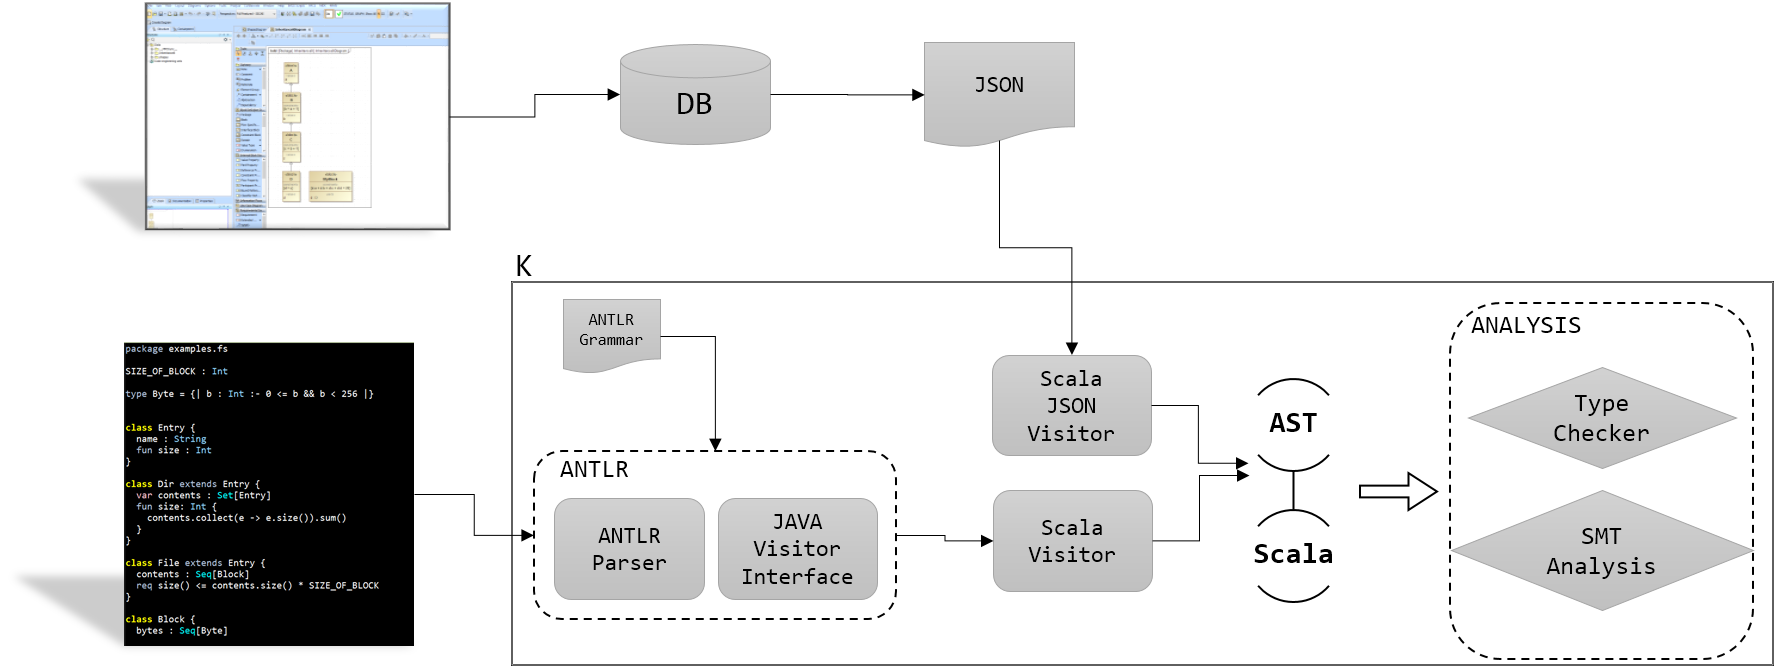
\includegraphics[scale=0.39]{K.png}
\caption{\Klang{}.}
\label{fig:k}
\end{figure*}

The typical scenario involves modelers creating SysML diagrams in a
tool such as MagicDraw and saving them to a central model
repository. This database of models is accessible via a REST API. The
input to the REST API is a unique identifier for a node (typically a
\sysml{} package) in the model, and the result is a list of all the
nodes that are part of the package specified in the input. The result
is provided as an array of JSON objects, where each object contains
information such as name, type, owner, etc. Typically, the types of
objects are classes, constraints, expressions, and member
properties. The \Klang{} tool chain takes this input and converts each
node in the list of nodes to a corresponding \Klang{} ASST
object. Since the list of nodes received from the REST API is
unordered and unstructured, we perform multiple passes on
the list of nodes. The first pass is performed to create the list of
classes in the model, followed by passes to populate properties and
constraints in each class. Once the \Klang{} model has been
constructed, the \Klang{} tool chain proceeds normally with type
checking and SMT analysis. Currently this scenario is based on a {\em
  pull} methodology where a modeler has to initiate the \Klang{} based
translation and analysis. In the future, we plan on automating this
effort and have it be executed on a regular cadence with results made
available through the model database to a web application.

\begin{figure*}
\centering
\fbox{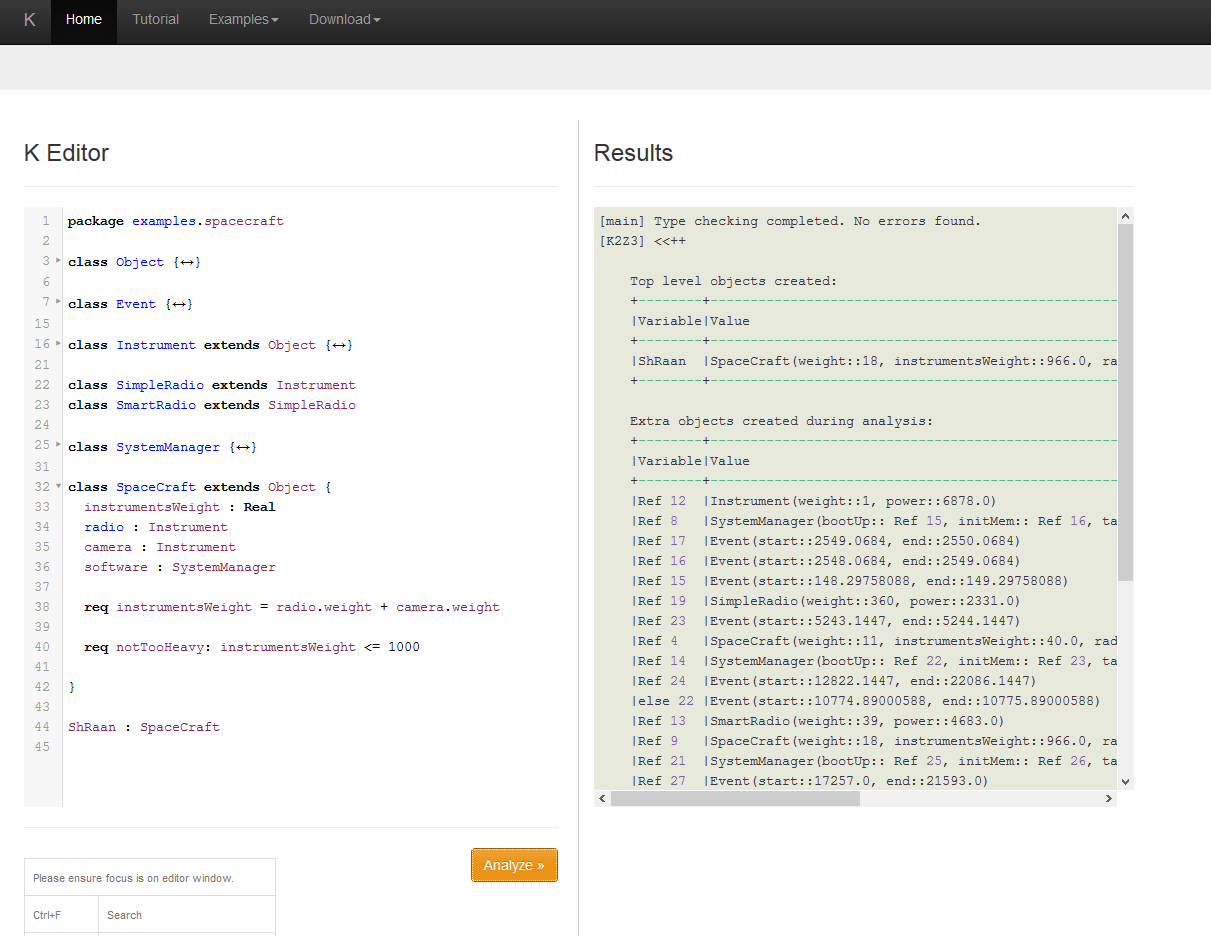
\includegraphics[scale=0.3]{kweb.png}}
\caption{\Klang{} editor in the browser.}
\label{fig:k}
\end{figure*}

A second common scenario for using \Klang{} is via the web browser. We
have created a simple HTML based \Klang{} code editor along with the
functionality to invoke the type checker and SMT analysis via the web
browser. This page is used for purposes of teaching, learning,
exploring, and prototyping with \Klang{}. The web page also provides a
tutorial, documentation, and \Klang{} examples as a guide. 

Finally, the \Klang{} tool chain is also available as a binary
download for all major operating systems. Users may download the tool
chain and invoke the \Klang{} parser, type checker, and SMT analyzer
from the command line.




\section{Related Work}
\label{sec:related-work}

\Klang{} is intended to represent a textual modeling language capable of representing \sysml{} concepts, specifically class diagrams with constraints.
However, as mentioned in the introduction, it also contains programming constructs.
As such it can be perceived as a wide-spectrum modeling/programming language.

Wide spectrum specification languages have been investigated to length in the formal 
methods community. One of the most well-known examples is \vdm{} 
\cite{vdm78,bjoerner-jones-82,jones90,jones-shaw-90}. \vdm{} in its
original form \cite{vdm78} provided a combination of procedural programming and
functional programming and specification using sets, lists and maps (with proper 
mathematical notation), and higher-order predicate logic. \vdmpp{} 
\cite{vdmplusplus05} added object-orientation to \vdm{}, which is now part of
the \vdm{} standard \cite{vdmsl}. The \raiselang{} specification language (\rsl{})
\cite{raise92} is a wide-spectrum language taking inspiration from \vdm{} as well as 
from other modeling languages such as \zlang{} and from algebraic specification 
languages, such as \clear{}. \asml{} \cite{asml05} is a more recent wide-spectrum
specification language, in many ways similar to \vdm{}, but based on the fundamental concept that operations operate on algebras.

Several high-level programming languages have been developed in recent years,
including  the early \sml{} (Standard ML) \cite{standard-ml-97}, its derivative
\ocaml{} \cite{ocaml}, and \haskell{} \cite{haskell}. However, also \java{}
can be considered high-level due to its libraries of collections (sets, lists, and 
maps), as well as the iterator concept. \python{} \cite{python} is close to 
combining object-oriented and functional programming. The 
\scala{} \cite{scala} language does this to the full extent, as does the
\fortress{} \cite{fortress}.

Specification constructs have been introduced in programming languages, in the form
of design-by-contract (pre/post conditions + class invariants). Examples are
\eiffel{} \cite{eiffel} and \specsharp{} \cite{specsharp}, where contracts are 
part of the language. \scala{} has library functions for writing pre/post conditions 
on functional programs \cite{odersky-rv10}. Finally, The \jml{} language \cite{jml} 
allows to write design-by-contract specifications for \java{} as comments. These are 
ignored by the standard \java{} compiler, and therefore must be processed with 
special tools. \eml{} (Extended ML) \cite{sannella-eml-97} takes a slightly different approach to specification and formal development of \sml{} programs.
\eml{} specifications look just like \sml{} programs except that axioms are allowed in signatures and in place of code in structures and functors. Some \eml{} specifications are executable, since \sml{} function definitions are just axioms of a certain special form. This makes EML a wide-spectrum language which can be used to express every stage in the development of a \sml{} program from the initial high-level specification to the final program itself and including intermediate stages in which specification and program are intermingled.

\notethis{References for Z and Clear.}.

\notethis{Other relevant literature, like C verification tools, diff tools, ...}

\notethis{What we do different.}


  
  
Model checking software:
  Java PathFinder 
    \cite{havelund-jpf-00}
    \cite{havelund-visser02}  
  \cite{holzmann-spin-2004}


\section{CONCLUSION}
\label{sec:conclusion}

We have presented an overview of the \Klang{} language in this
paper. \Klang{} is intended to be used in a modeling environment for
proving satisfiability of \sysml{} models and exploring solutions to
various types of specifications, such as structure,
planning/scheduling, etc. We have also presented in detail, our
methodology for performing automatic translation of \Klang{}
specifications to SMT-LIB, and using an SMT solver such as \zthree{}
to perform model finding. Using manual methods of creating \Klang{}
specifications from \sysml{} models and reference materials, we have
already observed \Klang{} provide value in the modeling environment by
discovering unsatisfiability of scheduling problems in the proposed
Europa Clipper mission concept, which was confirmed by external manual
analysis.  In our current experience, \Klang{} seems to be sufficient
for creating small to medium sized \sysml{} models and proving
properties about them.
%
Concerning problems faced, a main challenge of course is the
higher-order nature of K, requested by mission engineers
(expressiveness prioritized over guaranteed analyzability).  SMT-LIB
is generally first-order.  Some problems are a consequence of using
SMT-LIB solvers, which struggle with the combination of arrays (used
for the heap and for sets) and universal quantification. Additionally,
the use of Real numbers and arithmetic on them is also a known SMT
challenge, especially in the context of arrays.
%
We are now in the process of creating tools to automatically translate
\sysml{} models to \Klang{} specifications (and back) and perform analysis on
them using the \Klang{} infrastructure. This will make it possible to view
a model as graphics as well as in text. The translation of K needs to
be extended to cover more constructs, including statements with
side-effects. Other challenges is making K executable by translation
to Scala, including executing OCL-like expressions,
and providing support for reflection such that models can query themselves.



%\newpage

\bibliographystyle{apalike}
{\small \bibliography{biblio}}

%\appendix

%
\section{Grammar}
\label{sec:grammar}

\begin{verbatim}

grammar Model;

model:
    packageDeclaration?
    importDeclaration* 
    topDeclarationList? 
    EOF
  ;

topDeclarationList: topDeclaration (SEP topDeclaration)* SEP?
  ;

topDeclaration:
    memberDeclaration 
  | classDeclaration 
  | assocDeclaration 
  ;

packageDeclaration:
    'package' qualifiedName
  ;

importDeclaration:
    'import' qualifiedName ('.' '*')?
  ;

memberDeclarationList:
    memberDeclaration (SEP memberDeclaration)* SEP?
  ;

assocMemberDeclarationList:
    assocMemberDeclaration (SEP assocMemberDeclaration)* SEP?
  ;

classDeclaration:
    'class' Identifier typeParameters? extending? '{' memberDeclarationList? '}' 
  ;

assocDeclaration:
    'assoc' Identifier  '{' assocMemberDeclarationList? '}'
  ;

typeParameters:
      '[' typeParameter (',' typeParameter)* ']'
    ;

typeParameter:
      Identifier (':' typeBound)?
    ;

typeBound:
      type ('+' type)*
    ;
      
extending:
    'extends' type (',' type)*
  ;

type:
    primitiveType                   # PrimType
  | qualifiedName typeArguments?    # IdentType
  | type (tokenStar type)+          # CartesianType
  | type tokenArrow type            # FuncType
  | '{' type '}'                    # SetType
  | '[' type ']'                    # ListType
  | '<' type ',' type '>'           # MapType
  | '(' type ')'					# ParenType
  | '{|' Identifier ':' type  SUCHTHAT expression '|}' # SubType 
  | type '?' # OptionalType
  ;

expressionOrStar:
    expression
    | '*'
    ;

typeArguments:
    '[' type (',' type)* ']'
  ;

memberDeclaration:
    sortDeclaration 
  | typeDeclaration 
  | valueDeclaration 
  | variableDeclaration
  | functionDeclaration
  | constraint 
  | expression
  ;

assocMemberDeclaration:
    roleDeclaration
  | memberDeclaration
  ;

valueDeclaration:
    'val' pattern ('=' expression)? 
  ;

sortDeclaration:
    'type' Identifier 
  ;

typeDeclaration:
    'type' Identifier typeParameters? '=' type 
  ;

variableDeclaration:
    'var' pattern ('=' expression)? 
  ;

roleDeclaration:
    partDeclaration
  | refDeclaration
  ;

partDeclaration:
    'part' Identifier ':' Identifier multiplicity?
    ;

refDeclaration:
    'ref' Identifier ':' Identifier multiplicity?
    ;

multiplicity:
    expressionOrStar ('..' expressionOrStar)?
    ;

functionDeclaration:
    shortFunctionDeclaration
  | longFunctionDeclaration
  ;

shortFunctionDeclaration:
    'fun' Identifier ('(' patternList? ')')+ (':' type)? 
    '='
    expression
  ;

longFunctionDeclaration:
    'fun' Identifier ('(' patternList? ')')+ (':' type)? 
    functionSpecification*
    '{'
    memberDeclarationList?
    '}'
  ;

functionSpecification:
    'pre'  expression 
  | 'post' expression   
  ;

constraint:
    'req' (Identifier ':')?  expression
  ;

primitiveType:
    'Bool'
  | 'Char'
  | 'Int'       // Scala bigint (arbitrary precision)
  | 'Real'      // double
  | 'String'
  | 'Unit'  
  ;

tokenLessThan:
    '<' 
    | 'lt'
    ;
tokenGreatherThan:
    '>'
    | 'gt'
    ;
tokenLessThanEqual:
    '<='
| 'lte'
;
tokenGreaterThanEqual:
    '>='
    | 'gte'
    ;
tokenAnd:
    '&&' 
    | 'and'
    ;
tokenOr:
    '||'
    | 'or'
    ;
tokenNot:
    '!'
    | 'not'
    ;
tokenImplies:
    '=>'
    | 'implies'
    ;
tokenIFF:
    '<=>'
    | 'iff'
    ;
tokenEquals:
    '='
    | 'eq'
    ;
tokenStar:
    '*'
    ;
tokenArrow:
    '->'
    ;

tokenEnd: 
    'end' 
    ;
    
effect:
    expression (SEP expression)*
  ;
expression: 
    bracketedExpression # BracketedExp
  | literal #LiteralExp
  | Identifier #IdentExp
  | expression '.' Identifier #DotExp
  | expression '(' argumentList? ')' #AppExp
  | 'if' expression 'then' memberDeclarationList? ('else' memberDeclarationList?)? tokenEnd #IfExp
  | 'while' expression 'do' memberDeclarationList? tokenEnd #WhileExp
  | 'for' '(' pattern 'in' expression ')' 'do' memberDeclarationList? tokenEnd # ForExp 
  | 'match' expression 'with' match+ 'end' #MatchExp
  | tokenNot expression #NotExp
  | 'forall' rngBindingList SUCHTHAT expression #ForallExp 
  | 'exists' rngBindingList SUCHTHAT expression #ExistsExp 
  | '{' expressionList? '}' #SetEnumExp
  | '{' expression '..' expression '}' #SetRngExp
  | '{' expression '|' rngBindingList SUCHTHAT expression '}' #SetCompExp 
  | '[' expressionList? ']' #ListEnumExp
  | '[' expression '..' expression ']' #ListRngExp
  | '[' expression '|' pattern 'in' expression SUCHTHAT expression ']' #ListCompExp 
  | '<' mapPairList? '>' #MapEnumExp
  | '<' mapPair '|' rngBindingList SUCHTHAT expression '>' #MapCompExp 
  | expression ('*'|'/'|'%'|'inter'|'\\'|'++'|'#'|'^') expression #BinOp1Exp
  | expression ('+'|'-'|'union') expression #BinOp2Exp
  | expression 
      (
         tokenLessThanEqual | tokenGreaterThanEqual | tokenLessThan | tokenGreatherThan 
       | tokenEquals | tokenNot tokenEquals
       | 'isin'|'!isin'|'subset'|'psubset' 
      )  
    expression #BinOp3Exp
  | expression tokenAnd expression #AndExp
  | expression tokenOr expression #OrExp
  | expression (tokenImplies | tokenIFF) expression #IFFExp
  | expression ':=' expression #AssignExp
  | expression 'is' type # TypeCheckExp
  | expression 'as' type # TypeCastExp
  | 'assert' '(' expression ')' #AssertExp 
  | '~' expression #NegExp
  | pattern '->' expression #LambdaExp
  | 'continue' #ContinueExp
  | 'break' #BreakExp
  | 'return' expression? #ReturnExp
  | '$' #ResultExp
  ;

argumentList: 
    positionalArgumentList #PosArgList
  | namedArgumentList # NamedArgList
  ;

positionalArgumentList:
    expression (',' expression)* 
    ;

namedArgumentList:
   namedArgument (',' namedArgument)* 
  ;

namedArgument :
    Identifier '=' expression
  ;

bracketedExpression:
    '(' expression ')' #ParenExp
  | '(' expression (',' expression)+ ')' #TupleExp
  ;

idValueList:
    idValuePair (',' idValuePair)*
  ;

idValuePair:
    Identifier ':=' expression
  ;

match:
  'case' pattern ('|' pattern)* '=>' expression 
  ;

mapPairList:
    mapPair (',' mapPair)*
  ;

mapPair:
    expression ':' expression 
  ;

rngBindingList:
    rngBinding (',' rngBinding)*
  ;

rngBinding:
    patternList ':' collectionOrType
  ;

patternList:
    pattern (',' pattern)*
  ;

collectionOrType:
    expression
  | type
  ;
  
pattern:
    literal # LiteralPattern
  | '_' #DontCarePattern   
  | Identifier #IdentPattern
  | '(' pattern (',' pattern)+ ')' #CartesianPattern  
  | pattern ':' type # TypedPattern
  ;
  
identifierList:
    Identifier (',' Identifier)*
  ;

expressionList:
    expression (',' expression)*
  ;
    
qualifiedName:
    Identifier ('.' Identifier)*
  ;

literal:
    IntegerLiteral
  | FloatingPointLiteral
  | CharacterLiteral
  | StringLiteral
  | BooleanLiteral
  | NullLiteral
  | ThisLiteral
  ;

SUCHTHAT :
    '.' 
  ;

IntegerLiteral:
      DecimalIntegerLiteral
    |   HexIntegerLiteral
    |   OctalIntegerLiteral
    |   BinaryIntegerLiteral
    ;

fragment
DecimalIntegerLiteral:
      DecimalNumeral IntegerTypeSuffix?
    ;

fragment
HexIntegerLiteral:
      HexNumeral IntegerTypeSuffix?
    ;

fragment
OctalIntegerLiteral:
      OctalNumeral IntegerTypeSuffix?
    ;

fragment
BinaryIntegerLiteral:
      BinaryNumeral IntegerTypeSuffix?
    ;

fragment
IntegerTypeSuffix:
      [lL]
    ;

fragment
DecimalNumeral:
      '0'
    |   NonZeroDigit (Digits? | Underscores Digits)
    ;

fragment
Digits:
      Digit (DigitOrUnderscore* Digit)?
    ;

fragment
Digit:
      '0'
    |   NonZeroDigit
    ;

fragment
NonZeroDigit:
      [1-9]
    ;

fragment
DigitOrUnderscore:
      Digit
    |   '_'
    ;

fragment
Underscores:
      '_'+
    ;

fragment
HexNumeral:
      '0' [xX] HexDigits
    ;

fragment
HexDigits:
      HexDigit (HexDigitOrUnderscore* HexDigit)?
    ;

fragment
HexDigit:
      [0-9a-fA-F]
    ;

fragment
HexDigitOrUnderscore:
      HexDigit
    |   '_'
    ;

fragment
OctalNumeral:
      '0' Underscores? OctalDigits
    ;

fragment
OctalDigits:
      OctalDigit (OctalDigitOrUnderscore* OctalDigit)?
    ;

fragment
OctalDigit:
      [0-7]
    ;

fragment
OctalDigitOrUnderscore:
      OctalDigit
    |   '_'
    ;

fragment
BinaryNumeral:
      '0' [bB] BinaryDigits
    ;

fragment
BinaryDigits:
      BinaryDigit (BinaryDigitOrUnderscore* BinaryDigit)?
    ;

fragment
BinaryDigit:
      [01]
    ;

fragment
BinaryDigitOrUnderscore:
      BinaryDigit
    |   '_'
    ;

FloatingPointLiteral:
      DecimalFloatingPointLiteral
    |   HexadecimalFloatingPointLiteral
    ;

fragment
DecimalFloatingPointLiteral:
      Digits '.' Digits? ExponentPart? FloatTypeSuffix?
    |   '.' Digits ExponentPart? FloatTypeSuffix?
    |   Digits ExponentPart FloatTypeSuffix?
    |   Digits FloatTypeSuffix
    ;

fragment
ExponentPart:
      ExponentIndicator SignedInteger
    ;

fragment
ExponentIndicator:
      [eE]
    ;

fragment
SignedInteger:
      Sign? Digits
    ;

fragment
Sign:
      [+-]
    ;

fragment
FloatTypeSuffix:
      [fFdD]
    ;

fragment
HexadecimalFloatingPointLiteral:
      HexSignificand BinaryExponent FloatTypeSuffix?
    ;

fragment
HexSignificand:
      HexNumeral '.'?
    |   '0' [xX] HexDigits? '.' HexDigits
    ;

fragment
BinaryExponent:
      BinaryExponentIndicator SignedInteger
    ;

fragment
BinaryExponentIndicator:
      [pP]
    ;

BooleanLiteral:
      'true'
    |   'false'
    ;

NullLiteral:
  'null'
  ;

ThisLiteral:
  'this'
  ;

CharacterLiteral:
      '\'' SingleCharacter '\''
    |   '\'' EscapeSequence '\''
    ;

fragment
SingleCharacter:
      ~['\\]
    ;
    
StringLiteral:
      '"' StringCharacters? '"'
    ;

fragment
StringCharacters:
      StringCharacter+
    ;

fragment
StringCharacter:
      ~["\\]
    |   EscapeSequence
    ;

fragment
EscapeSequence:
      '\\' [btnfr"'\\]
    |   OctalEscape
    |   UnicodeEscape
    ;

fragment
OctalEscape:
      '\\' OctalDigit
    |   '\\' OctalDigit OctalDigit
    |   '\\' ZeroToThree OctalDigit OctalDigit
    ;

fragment
UnicodeEscape:
      '\\' 'u' HexDigit HexDigit HexDigit HexDigit
    ;

fragment
ZeroToThree:
      [0-3]
    ;

Identifier:
      JavaLetter JavaLetterOrDigit*
    ;

fragment
JavaLetter:
      [a-zA-Z$_] // these are the "java letters" below 0xFF
    |   // covers all characters above 0xFF which are not a surrogate
        ~[\u0000-\u00FF\uD800-\uDBFF]
        {Character.isJavaIdentifierStart(_input.LA(-1))}?
    |   // covers UTF-16 surrogate pairs encodings for U+10000 to U+10FFFF
        [\uD800-\uDBFF] [\uDC00-\uDFFF]
        {Character.isJavaIdentifierStart(Character.toCodePoint((char)_input.LA(-2), (char)_input.LA(-1)))}?
    ;

fragment
JavaLetterOrDigit:
      [a-zA-Z0-9$_] // these are the "java letters or digits" below 0xFF
    |   // covers all characters above 0xFF which are not a surrogate
        ~[\u0000-\u00FF\uD800-\uDBFF]
        {Character.isJavaIdentifierPart(_input.LA(-1))}?
    |   // covers UTF-16 surrogate pairs encodings for U+10000 to U+10FFFF
        [\uD800-\uDBFF] [\uDC00-\uDFFF]
        {Character.isJavaIdentifierPart(Character.toCodePoint((char)_input.LA(-2), (char)_input.LA(-1)))}?
    ;

fragment // ;; added this
CommentBegin:
    '---' '-'*
   | '===' '='* // to experiment with different ways of showing start of comment
   ;

fragment 
CommentEnd:
    '---' '-'*
   ;

COMMENT :
     CommentBegin .*? CommentEnd -> skip
  ;

LINE_COMMENT:
    '--' ~[\r\n]* -> skip
  ;

WS:
    [ \t\r\n\u000C]+ -> skip
  ;

SEP:
    ';'
  ;

SEPSEP:
    ';;'
  ;

\end{verbatim}


\end{document}
